\fancyhead[C]{\normalsize\textbf{$\qquad$ Teil II: Multiple-Choice}}
\section*{Aufgabe 2 (34 Punkte)}
\vspace{0.4cm}
\subsection*{\frage{1}{3}}
$ A $ und $ B $ seien zwei Aussagen. Die zusammengesetzte Aussage
\begin{align*}
	\neg (A \ \Rightarrow \ \neg B)
\end{align*}
ist äquivalent zu 
\renewcommand{\labelenumi}{(\alph{enumi})}
\begin{enumerate}
	\item $ A \vee B $.
	\item $ A \wedge B $.
	\item $ (\neg A) \vee (\neg B)$
	\item $ (\neg A) \wedge (\neg B)$.
\end{enumerate}\ \\
\textbf{Lösung:}
\begin{mdframed}
\underline{\textbf{Vorgehensweise:}}
\renewcommand{\labelenumi}{\theenumi.}
\begin{enumerate}
\item Löse die Aufgabe mithilfe einer Wahrheitstabelle.
\end{enumerate}
\end{mdframed}

\underline{1. Löse die Aufgabe mithilfe einer Wahrheitstabelle}\\
Eine Aussage kann nur die Wahrheitswerte wahr ($ W $) oder falsch ($ F $) annehmen.
Dementsprechend gibt es bei zwei Aussagen $ A $, $ B $ genau vier Kombinationsmöglichkeiten der Wahrheitswerte.
Aus diesen Kombinationen ergeben sich dann die Wahrheitswerte der verknüpften Aussagen.
\begin{center}
	\begin{tabular}{cllll}
		\hline
		\multicolumn{1}{c|}{$A$} & \multicolumn{4}{l}{$W$ $W$ $F$ $F$} \\
		\multicolumn{1}{c|}{$B$} & \multicolumn{4}{l}{$W$ $F$ $W$ $F$} \\ 
		\multicolumn{1}{c|}{$\neg A$} & \multicolumn{4}{l}{$F$ $F$ $W$ $W$} \\
		\multicolumn{1}{c|}{$\neg B$} & \multicolumn{4}{l}{$F$ $W$ $F$ $W$} \\
		\hline
		\multicolumn{1}{c|}{(a) \ \ $ A \vee B$} & \multicolumn{4}{l}{$W$ $W$ $W$ $F$} \\ 
		\multicolumn{1}{c|}{(b) \ \ $ A \wedge B$} & \multicolumn{4}{l}{$W$ $F$ $F$ $F$} \\ 
		\multicolumn{1}{c|}{(c) \ \ $ (\neg A) \vee (\neg B)$} & \multicolumn{4}{l}{$F$ $W$ $W$ $W$} \\
		\multicolumn{1}{c|}{(d) \ \ $ (\neg A) \wedge (\neg B)$} & \multicolumn{4}{l}{$F$ $F$ $F$ $W$} \\
		\hline
		\multicolumn{1}{c|}{$ A \Rightarrow B$} & \multicolumn{4}{l}{$W$ $F$ $W$ $W$} \\ 
		\multicolumn{1}{c|}{$ A \Rightarrow  \neg B$} & \multicolumn{4}{l}{$F$ $W$ $W$ $W$} \\ 
		\multicolumn{1}{c|}{$ \neg(A \Rightarrow  \neg B)$} & \multicolumn{4}{l}{$W$ $F$ $F$ $F$} \\ 
		\hline
	\end{tabular}
\end{center}
Damit ist Antwort (b) korrekt. \\
\\
Alternativ lässt sich die Antwort auch anders herleiten. Durch Umformungen erhalten wir:
\begin{align*}
	\neg (A \ \Rightarrow \ \neg B)
	&\Leftrightarrow
	\neg ((\neg A) \vee (\neg B))
	\Leftrightarrow
	\neg (\neg A) \wedge \neg(\neg B)
	\Leftrightarrow
	A \wedge B.
\end{align*}


\newpage

\subsection*{\frage{2}{2}}
Die Folge $ \lbrace a_n \rbrace_{n \in \N} $ ist monoton wachsend und konvergiert mit $ \lim_{n \to \infty} a_n = -2 $.
Die Folge $ \lbrace b_n \rbrace_{n \in \N} $ ist definiert durch $ b_n = (-3) \cdot a_n $.\\
\\
Dann folgt:
\renewcommand{\labelenumi}{(\alph{enumi})}
\begin{enumerate}
	\item $ \lbrace b_n \rbrace_{n \in \N} $ ist monoton wachsend und divergent.
	\item $ \lbrace b_n \rbrace_{n \in \N} $ ist monoton wachsend und konvergent.
	\item $ \lbrace b_n \rbrace_{n \in \N} $ ist monoton fallend und divergent.
	\item $ \lbrace b_n \rbrace_{n \in \N} $ ist monoton fallend und konvergent.
	\item $ \lbrace b_n \rbrace_{n \in \N} $ ist nicht monoton und divergent.
\end{enumerate}
\ \\
\textbf{Lösung:}
\begin{mdframed}
	\underline{\textbf{Vorgehensweise:}}
	\renewcommand{\labelenumi}{\theenumi.}
	\begin{enumerate}
		\item Leite die korrekte Antwort her.
	\end{enumerate}
\end{mdframed}
\underline{1. Leite die korrekte Antwort her}\\
Die konstante Folge $ (-3) $ ist konvergent. Demnach ist $ \lbrace b_n \rbrace_{n \in \N} $ als Produkt konvergenter Folgen konvergent.
Deswegen sind die Antworten (a),(c) und (e) falsch.
Die Folge $\lbrace a_n \rbrace_{n \in \N}$ ist monoton wachsend.
Damit folgt:
\begin{align*}
	a_n \leq a_{n+1}
	\ \Leftrightarrow \
	(-3) \cdot a_n = b_n \geq (-3 ) a_{n+1} = b_{n+1}.
\end{align*} 
Hierbei geht ein, dass sich die Richtung der Ungleichung bei negativem Vorzeichen ändert.\\
\\
Also ist $ \lbrace b_n \rbrace_{n \in \N} $ monoton fallend und somit Antwort (d) korrekt.
 

\newpage
\subsection*{\frage{3}{3}}
Eine Möbelfirma wirbt:
\begin{center}
	\glqq Wir schenken Ihnen die Mehrwertsteuer auf Ihren Möbelkauf\grqq
\end{center}
Die Mehrwertsteuer auf Möbel beträgt in der Schweiz $ 7.7 \% $.\\
Wie viel Prozent Rabatt gewährt also die Möbelfirma?
\renewcommand{\labelenumi}{(\alph{enumi})}
\begin{enumerate}
	\item 
	Es sind etwa $ 7.15 \% $.
	\item 
	Es sind etwa $ 7.56 \% $.
	\item 
	Es sind genau $ 7.7 \% $.
	\item
	Es sind etwa $ 7.78 \% $.
	\item
	Es sind etwa $ 8.34 \% $.
\end{enumerate}
\ \\
\textbf{Lösung:}
\begin{mdframed}
\underline{\textbf{Vorgehensweise:}}
\renewcommand{\labelenumi}{\theenumi.}
\begin{enumerate}
\item Bestimme den gewährten Rabatt.
\end{enumerate}
\end{mdframed}

\underline{1. Bestimme den gewährten Rabatt}\\
Angenommen wir kaufen ein Möbelstück im Wert von $ 100 $ (CHF).
Dann ist der Preis inklusive Mehrwertsteuer
\begin{align*}
	100 \cdot 1.077 = 107.7 \ \textrm{(CHF)}.
\end{align*} 
Den Rabatt erhalten wir durch:
\begin{align*}
	p \% = \frac{7.7}{107.7} 
	\approx 
	0.0715.
\end{align*}
Damit gewährt das Möbelhaus etwa einen Rabatt von $ 7.15 \% $.\\
\\
Also ist Antwort (a) korrekt.



\newpage

\subsection*{\frage{4}{3}}
Sei $ f $ eine Funktion einer reellen Variablen und $ x_0 \in D_f $.
$ x_0  $ heißt \textit{Fixpunkt von} $ f $, wenn gilt: $ f(x_0) = x_0 $.\\
\\
Welche der folgenden Aussagen ist wahr? 
\renewcommand{\labelenumi}{(\alph{enumi})}
\begin{enumerate}
	\item 
	Wenn $ f $ invertierbar ist, dann hat $ f $ keinen Fixpunkt.
	\item
	Wenn $ f $ invertierbar ist und $ f^{-1} $ mehrere Fixpunkte hat, dann hat $ f $ höchstens einen Fixpunkt.
	\item
	Wenn $ f $ invertierbar ist, dann hat $ f $ mindestens einen Fixpunkt.
	\item
	Wenn $ f  $ einen Fixpunkt hat, dann ist $ f $ invertierbar.
	\item
	Wenn $ f $ invertierbar ist und einen Fixpunkt hat, dann hat auch $ f^{-1} $ einen Fixpunkt.
\end{enumerate}
\ \\
\textbf{Lösung:}
\begin{mdframed}
\underline{\textbf{Vorgehensweise:}}
\renewcommand{\labelenumi}{\theenumi.}
\begin{enumerate}
\item Schließe falsche Antworten aus.
\end{enumerate}
\end{mdframed}

\underline{1. Schließe falsche Antworten aus}\\
Wir setzen für alle Beispiele $ D_f = \R $.
Wir betrachten die Funktion $ f(x) = x $. Diese Funktion hat unendlich viele Fixpunkte und ist invertierbar mit $ f^{-1}(x) = x =f(x) $. 
Deswegen sind die Antworten (a) und (b) falsch.\\
\\
Nun wählen wir $ f(x) = x + 1 $. Diese Funktion ist invertierbar und besitzt keinen Fixpunkt.
Deshalb ist Antwort (c) falsch.\\
\\
Die Funktion $ f(x) = |x| $ ist nicht invertierbar wegen $ f(-1) = f(1) $ und alle $ x \geq 0  $ sind Fixpunkte.
Damit ist die Antwort (d) falsch.\\
\\
Übrig bleibt Antwort (e). Wenn $ f  $ invertierbar ist und einen Fixpunkt hat, gilt: 
\begin{align*}
	f(x_0) = x_0 
	\ \Leftrightarrow \
	x_0 = f^{-1}(x_0).
\end{align*}
Hiermit können wir die korrekte Antwort (e) auch direkt bestimmen.

\newpage
\subsection*{\frage{5}{3}}
Seien $ a,b >0, \ b \neq 1 , \ n \in \N  $.\\
Welche der folgenden Identitäten ist allgemein gültig?
\renewcommand{\labelenumi}{(\alph{enumi})}
\begin{enumerate}
	\item 
	$ \log_{b^n}(a^n) = \frac{\log_{b}(a)}{n} $.
	\item 
	$ \log_{b^n}(a^n) = \sqrt[n]{\log_{b}(a)} $.
	\item
	$ \log_{b^n}(a^n) = \log_{b}(a) $.
	\item
	$ \log_{b^n}(a^n) = n \ \log_{b}(a) $.
	\item
	Keine der vorangehenden Aussagen ist im Allgemeinen gültig.
\end{enumerate}
\ \\
\textbf{Lösung:}
\begin{mdframed}
\underline{\textbf{Vorgehensweise:}}
\renewcommand{\labelenumi}{\theenumi.}
\begin{enumerate}
\item Verwende die Basisumrechnung des Logarithmus.
\end{enumerate}
\end{mdframed}

\underline{1. Verwende die Basisumrechnung des Logarithmus}\\
Mithilfe der Basisumrechnung des Logarithmus gilt allgemein:
\begin{align*}
	\log_{b^n}(a^n)
	=
	\frac{\log_{b}(a^n)}{\log_{b}(b^n)}
	=
	\frac{n \log_{b}(a)}{n \log_b(b)}
	=
	\frac{\log_b(a)}{\log_{b}(b)}
	=
	\log_{b}(a).
\end{align*}
Damit ist Antwort (c) korrekt.\\
\\
\textit{Anmerkung:}
Seien $a,b>0$ beliebig. Der Logarithmus zur Basis $ b $ lässt sich über eine andere Basis $ a $ folgendermaßen berechnen:
\begin{align*}
	\log_b(x) = \frac{\log_a(x)}{\log_a(b)}.
\end{align*}


 \newpage

\subsection*{\frage{6}{3}}
Ein Bergsteiger startet bei seinem Auto bei Sonnenaufgang um $ 5 $ Uhr mit dem Aufstieg und erreicht auf direktem Weg ohne Pause die Hütte um $ 13 $ Uhr.
Am anderen Tag geht er den genau gleichen Weg zurück; er startet um $ 8 $ Uhr und geht ohne anzuhalten. So erreicht er sein Auto um $12$:$50$ Uhr.\\
\\
Gibt es einen Tageszeitpunkt, zu dem er auf dem Weg aufwärts bzw. auf dem Weg abwärts an der gleichen Stelle ist? 
\renewcommand{\labelenumi}{(\alph{enumi})}
\begin{enumerate}
	\item 
	Ja, es gibt genau einen solchen Zeitpunkt.
	\item 
	Nein.
	\item
	Es kann sein, muss aber nicht sein.
	\item
	Es kann auch mehrere Zeitpunkte geben.
\end{enumerate}
\ \\
\textbf{Lösung:}
\begin{mdframed}
\underline{\textbf{Vorgehensweise:}}
\renewcommand{\labelenumi}{\theenumi.}
\begin{enumerate}
\item Überlege dir eine Modellierung dieser Fragestellung.
\item Finde die korrekte Antwort.
\end{enumerate}
\end{mdframed}

\underline{1. Überlege dir eine Modellierung dieser Fragestellung}\\
Wir nehmen an, dass sich das Auto auf der Höhe $ 0 $ und die Hütte auf der Höhe $ 1 $ befindet. Da der Bergsteiger für den Hin-und Rückweg den gleichen Weg ohne Pause wählt, können wir den zurückgelegten Weg in Abhängigkeit von der Zeit mit Geraden modellieren.
Mit $ g_1 $ bezeichnen wir die Gerade für den Hinweg. Diese wird definiert durch:
\begin{align*}
	g_1(5\mathrm{:}00) = 0 \ \textrm{und} \ g_1(13\mathrm{:}00) = 1. 
\end{align*}
Sei $ g_2 $ die Gerade für den Rückweg. Diese wird definiert durch:
\begin{align*}
	g_2(8\mathrm{:}00) = 1 \ \textrm{und} \ g_2(12\mathrm{:}50) = 0.
\end{align*}
\ \\
\underline{2. Finde die korrekte Antwort}\\
Der Tageszeitpunkt, zu dem er auf dem Weg aufwärts bzw. auf dem Weg abwärts an der gleichen Stelle ist, ist ein Schnittpunkt der Geraden $ g_1 $ und $ g_2 $.
Nun kann für zwei Geraden nur eine der folgenden Tatsachen gelten:
\begin{itemize}
	\item Die Geraden haben einen Schnittpunkt.
	\item Die Geraden haben keinen Schnittpunkt.
	\item Die Geraden haben unendlich viele Schnittpunkte.
\end{itemize}
Deswegen bestimmen wir nun die Steigung von $ g_1 $ und $ g_2 $:
\begin{align*}
	m_1 &= \frac{g_1(13\mathrm{:}00) - g_1(5\mathrm{:}00)}{13\mathrm{:}00 - 5\mathrm{:}00}
	=
	\frac{1 - 0}{8\ \mathrm{h}} = \frac{1}{8\ \mathrm{h}}\\
	m_2 &= \frac{g_2(12\mathrm{:}50) - g_2(08\mathrm{:}00)}{12\mathrm{:}50 - 8\mathrm{:}00}
	=
	\frac{0 - 1}{4\mathrm{:}50 \ \mathrm{h}}
	=
	\frac{- 1}{4\mathrm{:}50 \ \mathrm{h}}.
\end{align*}
Das $ \mathrm{h} $ soll verdeutlichen, dass es sich um einen Zeitraum und keine Uhrzeit handelt. Wegen $ m_1 > 0 $ und $ m_2 < 0 $ sind die Geraden nicht parallel bzw. liegen nicht aufeinander. Deswegen kann nur ein Schnittpunkt vorliegen.\\
Da der Zeitraum des Rückwegs innerhalb des Zeitraums des Hinweges befindet, gibt es genau einen Zeitpunkt an welchem sich die Wege schneiden.\\
\\
Damit ist Antwort (a) korrekt.\\
 


\newpage
\subsection*{\frage{7}{3}}
Gegeben ist die Funktion $ f $ definiert durch
\begin{align*}
	f(x) = \sin(x) + \cos(x)
\end{align*}
mit Definitionsgebiet $ D_f \in \R $. Für den Wertebereich $ W_f $ von $ f $ gilt:
\renewcommand{\labelenumi}{(\alph{enumi})}
\begin{enumerate}
	\item 
	$ W_f = [-1,1] $.
	\item
	$ W_f = [-\sqrt{2},\sqrt{2}] $.
	\item
	$ W_f = [-2,2] $.
	\item
	$ W_f = [0,2] $.
	\item
	$ W_f = [-\nicefrac{\pi }{2}, \nicefrac{\pi }{2}] $.
\end{enumerate}
\ \\
\textbf{Lösung:}
\begin{mdframed}
\underline{\textbf{Vorgehensweise:}}
\renewcommand{\labelenumi}{\theenumi.}
\begin{enumerate}
\item Bestimme lokale Minima und Maxima.
\end{enumerate}
\end{mdframed}

\underline{1. Bestimme lokale Minima und Maxima}\\
Um den Wertebereich bestimmen werden wir  die lokalen Minima und Maxima von $ f $ betrachten. Die erste Ableitung ist:
\begin{align*}
	f^\prime(x) = \cos(x) - \sin(x).
\end{align*}
Die kritischen Stellen erhalten wir wegen
\begin{align*}
	\cos(x) - \sin(x) = 0 \ \Leftrightarrow \
	\sin(x) = \cos(x)
\end{align*}
an den Schnittpunkten des Sinus und Kosinus.
\begin{center}
	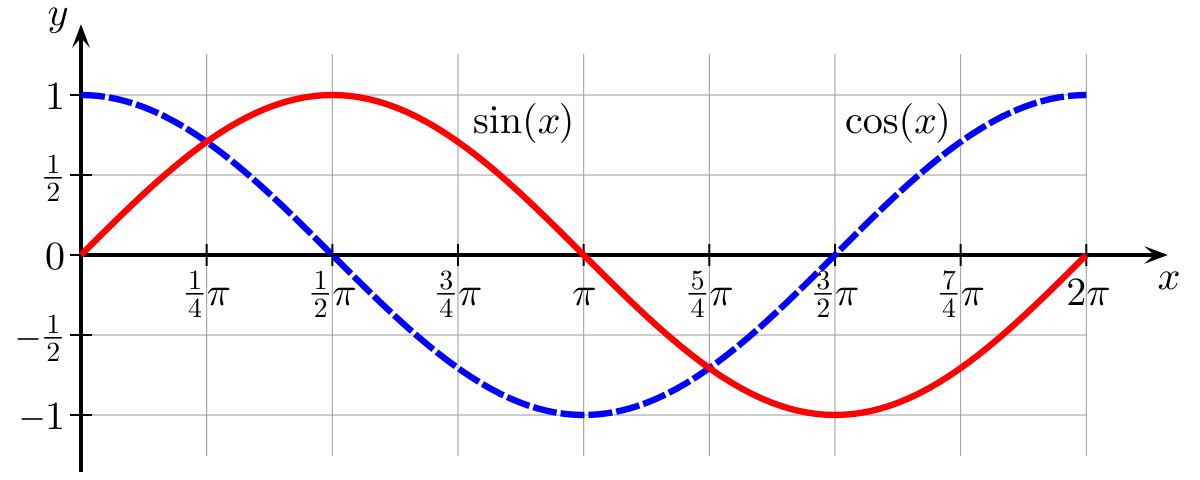
\includegraphics[scale=0.3]{pictures/Sinus_Kosinus_Kurve}
\end{center}
Da $ f $ periodisch ist, werden uns auf $ D_f = [0,2\pi] $ einschränken.
Mögliche Kandidaten für Extrempunkte sind:
\begin{align*}
	x_0 &= \frac{\pi}{4}\\
	x_1 &= \frac{\pi }{4} + \pi= \frac{5 \pi}{4}.
\end{align*}
Die zweite Ableitung ist:
\begin{align*}
	f^{\prime \prime} (x) = -\sin(x) - \cos(x) = -f(x). 
\end{align*}
Eingesetzt erhalten wir:
\begin{align*}
	f^{\prime \prime} (x_0) &= -\frac{\sqrt{2}}{2} - \frac{\sqrt{2}}{2} = -\sqrt{2} < 0\\
	f^{\prime \prime} (x_1) &= -\left(-\frac{\sqrt{2}}{2}\right) - \left(-\frac{\sqrt{2}}{2}\right) = \sqrt{2} >0.\\
\end{align*}
\begin{center}
	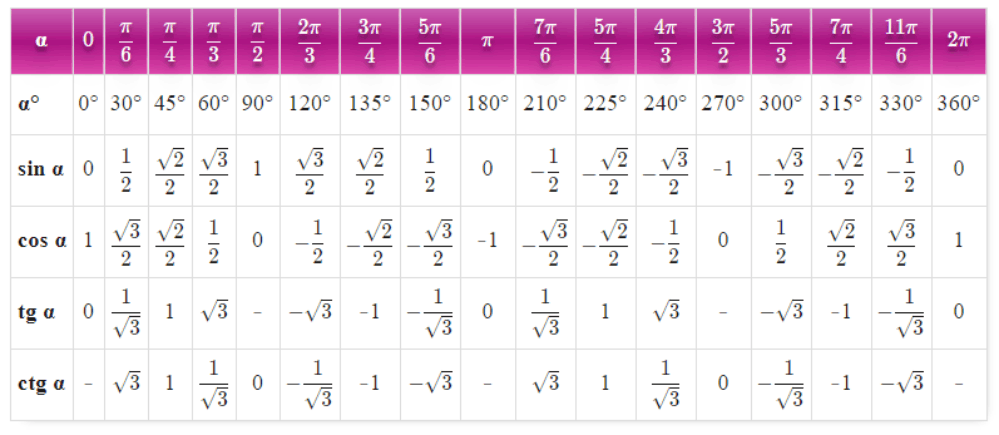
\includegraphics[scale=1.3]{pictures/Tabelle}
\end{center}
Wegen $ f(x_0) = \sqrt{2} $ und $ f(x_1) = -\sqrt{2} $ ist der Wertebereich $ W_f = [-\sqrt{2}, \sqrt{2}] $.\\
\\
Damit ist Antwort (b) korrekt.



\newpage

\subsection*{\frage{8}{3}}
$ f $ und $ g $ seien ungerade, differenzierbare Funktionen. Dann gilt:
\renewcommand{\labelenumi}{(\alph{enumi})}
\begin{enumerate}
	\item 
	$ f^\prime + g^\prime $ ist ungerade.
	\item
	$ f^\prime + g^\prime $ ist gerade.
	\item
	$ f^\prime \cdot g^\prime $ ist ungerade.
	\item
	Keine der obigen Antworten ist im Allgemeinen richtig.
\end{enumerate}
\ \\
\textbf{Lösung:}
\begin{mdframed}
\underline{\textbf{Vorgehensweise:}}
\renewcommand{\labelenumi}{\theenumi.}
\begin{enumerate}
\item Leite die Antwort mithilfe der Kettenregel her.
\end{enumerate}
\end{mdframed}

\underline{1. Leite die Antwort mithilfe der Kettenregel her}\\
Sei $ h  $ eine ungerade, differenzierbare Funktion.
Dann gilt
\begin{align*}
	h(x) = -h(-x)
	\ \Rightarrow \
	h^\prime (x) = (-1) \cdot (-1) \cdot h^\prime(-x) = h^\prime(-x)
\end{align*}
für alle $ x \in D_h $. Das bedeutet, dass die Ableitung einer ungeraden Funktion gerade ist.\\
\\
\textit{Frage: Was gilt dann für die Ableitung einer geraden Funktion?}\\
\\
Wegen 
\begin{align*}
	(f+g)(x) = f(x) +g(x) =-f(-x) - g(-x)
	=-(f(-x) + g(-x))= -(f+g)(-x)
\end{align*}
ist auch die Summe zweier ungerader Funktion ungerade. Aufgrund von 
\begin{align*}
	(f+g)^\prime = f^\prime + g^\prime
\end{align*}
ist $ f^\prime + g^\prime $ gerade (Weil $ f+g $ ungerade ist).\\
\\
Damit ist Antwort (b) korrekt.


\newpage
\subsection*{\frage{9}{2}}
Wir betrachten die differenzierbaren Funktionen $ f(x) $ und $ g(x) $, wobei $ g(x) > 0 $ für $ x \in \R $ gelte. Die Ableitung der Funktion
\begin{align*}
	k(x)
	=
	\frac{f(g(x))}{g(f(x))}
\end{align*}
ist dann
\renewcommand{\labelenumi}{(\alph{enumi})}
\begin{enumerate}
	\item 
	$ k^\prime(x) = \frac{f^\prime(g(x))g(f(x)) + f(g(x))g^\prime(f(x))}{(g(f(x)))^2} $.
	\item
	$ k^\prime(x) = \frac{f^\prime(g(x))g^\prime(x) }{g^\prime(f(x))f^\prime(x)} $.
	
	\item
	$ k^\prime(x) = 
	\frac{f^\prime(g(x))g^\prime(x)g(f(x)) - f(g(x)) g^\prime(f(x)) f^\prime(x) }
	{(g(f(x)))^2} $.
	\item
	$ k^\prime(x) = \frac{f^\prime(g(x))g(f(x)) - f(g(x))g^\prime(f(x))}{(g(f(x)))^2} $.
\end{enumerate}
\ \\
\textbf{Lösung:}
\begin{mdframed}
	\underline{\textbf{Vorgehensweise:}}
	\renewcommand{\labelenumi}{\theenumi.}
	\begin{enumerate}
		\item Verwende die Quotientenregel.
	\end{enumerate}
\end{mdframed}

\underline{1. Verwende die Quotientenregel}\\
Nach der Quotientenregel gilt:
\begin{align*}
	k^\prime(x)
	=
	\frac{(f(g(x)))^\prime g(f(x)) - f(g(x)) (g(f(x)))^\prime}{(g(f(x)))^2}
	=
	\frac{f^\prime(g(x)) \cdot g^\prime(x) \cdot g(f(x))
		- 
		f(g(x)) g^\prime(f(x)) \cdot f^\prime(x)
		}{(g(f(x)))^2}.
\end{align*}
Damit ist Antwort (c) korrekt.


\newpage
\subsection*{\frage{10}{3}}
Gegeben ist die Funktion
\begin{align*}
	f \ : \ \R \rightarrow \R, \ x \mapsto y = x \cdot |x| 
\end{align*}
Dann folgt:
\renewcommand{\labelenumi}{(\alph{enumi})}
\begin{enumerate}
	\item 
	$ f $ ist überall stetig und differenzierbar.
	\item
	$ f $ ist stetig in $ x_0 = 0 $, aber nicht differenzierbar in $ x_0 = 0 $.
	\item
	$ f $ ist differenzierbar in $ x_0 = 0 $, aber nicht stetig in $ x_0 = 0 $.
	\item
    $ f $ ist nicht stetig und nicht differenzierbar in $ x_0 = 0 $.
\end{enumerate}
\ \\
\textbf{Lösung:}
\begin{mdframed}
	\underline{\textbf{Vorgehensweise:}}
	\renewcommand{\labelenumi}{\theenumi.}
	\begin{enumerate}
		\item Verwende den Differenzenquotienten.
	\end{enumerate}
\end{mdframed}

\underline{1. Verwende den Differenzenquotienten}\\
Da $ f $ ein Produkt stetiger Funktionen ist, ist $ f $ selbst überall stetig.
Damit können wir die Antworten (c) und (d) ausschließen.\\
\\
Wir müssen nun klären, ob $ f $ in $ x_0 = 0 $ differenzierbar ist. Hierfür betrachten wir den Differenzenquotient:
\begin{align*}
	\frac{f(x) - f(x_0)}{x - x_0 } = \frac{x \cdot |x|}{x} = |x|.
\end{align*}
Eine Funktion heißt differenzierbar in $ x_0 $, wenn der Grenzwert
\begin{align*}
	\lim \limits_{x \to x_0} \frac{f(x) - f(x_0)}{x - x_0 }
\end{align*}
existiert. In unserem Fall gilt:
\begin{align*}
	\lim \limits_{x \to x_0} \frac{f(x) - f(x_0)}{x - x_0 }
	=
	\lim \limits_{x \to 0} |x| = 0.
\end{align*}
Damit ist $ f  $ in $ x_0 = 0 $ differenzierbar.\\
\\
Also ist Antwort (a) korrekt.

\newpage

\subsection*{\frage{11}{3}}
Das Taylorpolynom $ 4 $. Ordnung in $ x_0 = 0 $ der Funktion
\begin{align*}
	f(x) = e^{x^3}
\end{align*}
lautet:
\renewcommand{\labelenumi}{(\alph{enumi})}
\begin{enumerate}
	\item 
	$ P_4(x) = \frac{x^4}{4} + \frac{x^3}{3} + \frac{x^2}{2} + x $. 
	\item
	$ P_4(x) = \frac{x^4}{4} + \frac{x^3}{3} + \frac{x^2}{2} - x $. 
	\item
	$ P_4(x) = x^3 + x^2 + x + 2$. 
	\item
	$ P_4(x) = \frac{x^4}{4} + \frac{x^3}{3} + \frac{x^2}{2} + x +1 $. 
	\item
	$ P_4(x) = x^3 + 1$. 
	\item
	$ P_4(x) = \frac{x^4}{4} - \frac{x^3}{3} + \frac{x^2}{2} - x + 2 $. 
\end{enumerate}
\ \\
\textbf{Lösung:}
\begin{mdframed}
	\underline{\textbf{Vorgehensweise:}}
	\renewcommand{\labelenumi}{\theenumi.}
	\begin{enumerate}
		\item Verwende die Struktur der Ableitungen.
	\end{enumerate}
\end{mdframed}

\underline{1. Verwende die Struktur der Ableitungen.}\\
Wir betrachten die Ableitungen bis zur vierten Ordnung:
\begin{align*}
	f^{(0)}(x) &= e^{x^3}\\
	f^{(1)}(x) &= 3x^2 e^{x^3}\\
	f^{(2)}(x) &= 6x e^{x^3} + 3x^2 \cdot 3x^2 e^{x^3} = (9x^4 + 6x) e^{x^3}\\
	f^{(3)}(x) &= (36x^3+ 6) e^{x^3} + (9x^4 + 6x) \cdot 3 x^2 e^{x^3} 
	= (27x^6 + 54x^3 + 6) e^{x^3}\\
	f^{(4)}(x) &= (27 \cdot 6\cdot x^5+54 \cdot 3 \cdot x^2) e^{x^3}
	+ (27x^6 + 54x^3 + 6)\cdot 3 x^2 e^{x^3}.
\end{align*}
Spannend für uns ist, was für diese Ableitungen an $ x_0 = 0 $ passiert.
Es gilt $ f^{(1)}(0) = f^{(2)}(0) = f^{(4)}(0) = 0  $ und $ f^{(0)}(0) = 1 $ bzw. $ f^{(3)}(0) = 6 $.
Damit können die Antworten (a)--(d) und (f) nicht das korrekte Taylorpolynom sein und Antwort (e) ist korrekt.

\newpage

\subsection*{\frage{12}{3}}
Die Funktion zweier Variablen $ f $ ist homogen vom Grad $ 3 $ und die Funktion zweier Variablen $ g $ ist homogen vom Grade $ -3 $.\\
\\
Die Funktion $ h $ ist definiert durch
\begin{align*}
	h(x,y) = f(g(x,y),g(x,y)).
\end{align*}
Dann gilt:
\renewcommand{\labelenumi}{(\alph{enumi})}
\begin{enumerate}
	\item 
	$ h $ ist homogen vom Grad $ -1 $. 
	\item
	$ h $ ist homogen vom Grad $ 0 $. 
	\item
	$ h $ ist homogen vom Grad $ 6 $. 
	\item
	$ h $ ist homogen vom Grad $ -9 $.  
	\item
	$ h $ ist nicht homogen.
\end{enumerate}
\ \\
\textbf{Lösung:}
\begin{mdframed}
	\underline{\textbf{Vorgehensweise:}}
	\renewcommand{\labelenumi}{\theenumi.}
	\begin{enumerate}
		\item Verwende die Definition der Homogenität.
	\end{enumerate}
\end{mdframed}

\underline{1. Verwende die Definition der Homogenität}\\
Wir betrachten für $ \lambda \in \R $:
\begin{align*}
	h(\lambda \cdot x, \lambda \cdot y)
	&=
	f(g(\lambda \cdot x,\lambda \cdot y),g(\lambda \cdot x,\lambda \cdot y))
	=
	f(\lambda^{-3}g(x,y),\lambda^{-3} g(x,y))\\
	&=
	(\lambda^{-3})^3 f(g(x,y),g(x,y))
	=
	\lambda^{-9} h(x,y).
\end{align*}
Damit ist $ h $ homogen vom Grad $ -9 $.\\
\\
Also ist Antwort (d) korrekt.